\documentclass[11pt]{article}

\usepackage[T1]{fontenc}
\usepackage{lmodern}
\usepackage[margin=0.82in]{geometry}
\usepackage{microtype}
\usepackage{amsmath,amssymb,mathtools}
\usepackage{booktabs,tabularx,array}
\usepackage{graphicx}
\usepackage[dvipsnames]{xcolor}
\usepackage{tikz}
\usetikzlibrary{arrows.meta,positioning,calc}
\usepackage{enumitem}
\usepackage{fancyhdr}
\usepackage{hyperref}

\definecolor{AimBlue}{HTML}{155E75}
\definecolor{AimTeal}{HTML}{0F766E}
\definecolor{AimGold}{HTML}{B7791F}
\definecolor{AimInk}{HTML}{17202A}
\definecolor{AimSoft}{HTML}{F2F7F7}
\definecolor{AimRule}{HTML}{C8D8D8}
\definecolor{AimRed}{HTML}{9B2C2C}

\hypersetup{
  colorlinks=true,
  linkcolor=AimBlue,
  urlcolor=AimTeal,
  citecolor=AimBlue,
  pdftitle={PenroseAim: Optimal-Transport Flow Matching with Markov Inness Reveals},
  pdfauthor={Technical note generated from the PenroseAim implementation}
}

\setlength{\parindent}{0pt}
\setlength{\parskip}{0.55em}
\setlist[itemize]{leftmargin=1.25em,itemsep=0.15em,topsep=0.25em}
\setlist[enumerate]{leftmargin=1.35em,itemsep=0.2em,topsep=0.25em}
\renewcommand{\arraystretch}{1.18}

\pagestyle{fancy}
\fancyhf{}
\fancyhead[L]{\small\color{AimBlue}\textsc{PenroseAim}}
\fancyhead[R]{\small\color{AimInk}Hybrid continuous-time generative process}
\fancyfoot[C]{\small\color{AimInk}\thepage}
\renewcommand{\headrulewidth}{0.4pt}

\newcommand{\R}{\mathbb{R}}
\newcommand{\E}{\mathbb{E}}
\newcommand{\Pp}{\mathbb{P}}
\newcommand{\Ber}{\operatorname{Bern}}
\newcommand{\Bin}{\operatorname{Bin}}
\newcommand{\sigmoid}{\operatorname{sigmoid}}
\newcommand{\1}{\mathbf{1}}
\newcommand{\given}{\,\middle|\,}
\newcommand{\code}[1]{\texttt{#1}}
\newcommand{\term}[1]{\textcolor{AimBlue}{\textbf{#1}}}

\newenvironment{takeaway}
  {\begin{center}\begin{minipage}{0.92\linewidth}
   \color{AimInk}\hrule height 1.2pt\relax\vspace{0.45em}
   \textcolor{AimTeal}{\textbf{Key point.}}\ }
  {\vspace{0.35em}\hrule height 0.4pt\relax
   \end{minipage}\end{center}}

\begin{document}

\hypersetup{pageanchor=false}
\begin{titlepage}
\thispagestyle{empty}
\vspace*{1.0cm}
{\color{AimBlue}\rule{\linewidth}{2.2pt}}
\vspace{0.7cm}

{\Huge\bfseries\color{AimInk} PenroseAim\par}
\vspace{0.25cm}
{\LARGE\color{AimBlue} Optimal-Transport Flow Matching\\
with Markov Inness Reveals\par}

\vspace{0.7cm}
{\large A mathematical account of the implemented hybrid process for
\((x,y,\theta)\) geometry and discrete tile occupancy\par}

\vfill

\begin{center}
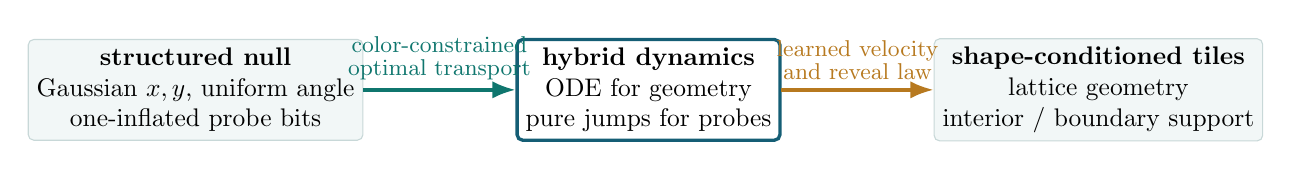
\begin{tikzpicture}[x=1cm,y=1cm,>=Latex,scale=0.92,transform shape]
  \node[draw=AimRule,fill=AimSoft,rounded corners=2pt,
        minimum width=3.15cm,minimum height=1.15cm,align=center] (source)
        {\textbf{structured null}\\Gaussian \(x,y\), uniform angle\\one-inflated probe bits};
  \node[draw=AimBlue,very thick,rounded corners=2pt,
        minimum width=3.25cm,minimum height=1.15cm,align=center,right=2.1cm of source] (hybrid)
        {\textbf{hybrid dynamics}\\ODE for geometry\\pure jumps for probes};
  \node[draw=AimRule,fill=AimSoft,rounded corners=2pt,
        minimum width=3.15cm,minimum height=1.15cm,align=center,right=2.1cm of hybrid] (data)
        {\textbf{shape-conditioned tiles}\\lattice geometry\\interior / boundary support};
  \draw[->,very thick,AimTeal] (source) -- node[above,align=center]
        {\small color-constrained\\[-1mm]\small optimal transport} (hybrid);
  \draw[->,very thick,AimGold] (hybrid) -- node[above,align=center]
        {\small learned velocity\\[-1mm]\small and reveal law} (data);
\end{tikzpicture}
\end{center}

\vfill

\begin{tabularx}{\linewidth}{@{}>{\bfseries\color{AimBlue}}l X@{}}
Scope & \code{PenroseAim} and the relevant \code{PenroseSpur} sampling/matching code\\
Implementation snapshot & 16 August 2026\\
Default experiment & hex symmetry, \(N=120\) returned tile tokens, L2 flow loss\\
Schedule convention & linear path time \(t\in[0,1]\) for training and sampling\\
Interpretation & continuous normalizing flow \(+\) time-inhomogeneous jump process\\
\end{tabularx}

\vspace{0.55cm}
{\color{AimBlue}\rule{\linewidth}{2.2pt}}
\end{titlepage}
\hypersetup{pageanchor=true}

\tableofcontents
\newpage

\section{Executive picture}

PenroseAim generates a set of colored tiles conditioned on an MPEG7 shape class.
Each tile carries two different kinds of state:
\[
  \underbrace{g_i=(x_i,y_i,a_i)\in\R^3}_{\text{continuous geometry}},
  \qquad
  \underbrace{b_i=(b_{i1},\ldots,b_{im})\in\{0,1\}^m}_{\text{identified inness probes}},
\]
where \(a_i=(\sqrt{3}/\pi)\,\operatorname{wrap}_{[-\pi,\pi)}(\theta_i)\).
The scale makes a uniform physical angle have unit variance, just like the
Gaussian source coordinates \(x\) and \(y\).

The model is best understood as a \term{piecewise-deterministic Markov process}
(PDMP):
\begin{itemize}
  \item \(g_i\) moves continuously under a learned flow-matching velocity;
  \item each probe \(b_{ij}\) is revealed at one random continuous time and is
        then frozen;
  \item an exact linear-sum assignment supplies a low-cost, color-preserving
        coupling between source and data geometry before interpolation.
\end{itemize}

\begin{takeaway}
In this note, ``diffusion'' does not mean Brownian motion, a DDPM, or an SDE.
The geometry is a deterministic probability flow (conditional flow matching);
the inness component is a pure-jump Markov construction.  The combination is
continuous in time but not continuous in every state coordinate.
\end{takeaway}

\section{Data state and notation}

\subsection{Tile probes and soft inness}

PenroseSpur tests the tile center and every vertex against a target mask.
Thus \(m=V+1\): \(m=7\) for a hexagon and \(m=5\) for a Penrose rhombus.
For target tile \(i\), let \(r_{ij}\in[0,1]\) be the sampled mask value at
probe \(j\).  The training data contain
\[
  \omega_i=\frac1m\sum_{j=1}^m r_{ij}\in[0,1],
  \qquad
  b^1_{ij}=\1\{r_{ij}>1/2\}.
\]
The real-valued \(\omega_i\) is used only as a geometry-loss weight.  The
binary vector \(b_i^1\) is the endpoint of the discrete generative process.
Because masks can have soft edge pixels, \(\omega_i\) need not equal
\(m^{-1}\sum_j b^1_{ij}\).  At generation time, however, displayed opacity is
\[
  \widehat\omega_i=\frac1m\sum_{j=1}^m \widehat b_{ij}.
\]

PenroseSpur ranks all mother-canvas tiles by \(\omega_i\) (with tiny random
tie-breaking noise) and retains the best \(N\).  Consequently, the learned
distribution is the distribution of the \emph{top-\(N\) selected set}, not the
unfiltered mother canvas.

\subsection{Complete conditional state}

For one example, write
\[
  G=(g_1,\ldots,g_N)\in\R^{N\times3},\qquad
  B=(b_{ij})\in\{0,1\}^{N\times m}.
\]
The conditioning variables are tile colors \(C=(c_1,\ldots,c_N)\), with
\(c_i\in\{0,1\}\), and the shape-class label \(\ell\).  A Direct Transformer
maps
\[
  (G_t,B_t,C,t,\ell)\longmapsto
  \bigl(v_\theta(G_t,B_t,C,t,\ell),\;
        \eta_\theta(G_t,B_t,C,t,\ell)\bigr),
\]
where \(v_\theta\in\R^{N\times3}\) is geometry velocity and
\(\eta_\theta\in\R^{N\times m}\) contains clean-probe logits.  Tile tokens share
self-attention with learned global tokens; color, class, and sinusoidal time
embeddings provide conditioning.

\section{The structured source distribution}

\subsection{Geometry null}

The source geometry is factorized over tiles:
\[
  x_i^0,y_i^0\overset{\text{iid}}{\sim}\mathcal N(0,1),
  \qquad
  a_i^0\sim\mathcal U[-\sqrt3,\sqrt3).
\]
The angle source corresponds to \(\theta_i^0\sim\mathcal U[-\pi,\pi)\).

\subsection{One-inflated Bernoulli null for probes}

The discrete source preserves the empirical tendency for a retained tile to
be completely interior.  Independently for each tile, draw
\[
  F_i\sim\Ber(\rho),\qquad E_{ij}\overset{\text{iid}}{\sim}\Ber(p),
  \qquad b^0_{ij}=F_i\lor E_{ij}.
\]
Equivalently,
\[
q_0(b_i)=
  \rho\,\1\{b_i=\mathbf1_m\}
  +(1-\rho)\prod_{j=1}^m p^{b_{ij}}(1-p)^{1-b_{ij}}.
\]
For the count \(K_i=\sum_j b^0_{ij}\),
\[
 \Pp(K_i=k)=
 \begin{cases}
 (1-\rho)\binom{m}{k}p^k(1-p)^{m-k},&k<m,\\
 \rho+(1-\rho)p^m,&k=m.
 \end{cases}
\]
PenroseAim fits \((\rho,p)\) by maximum likelihood to count histograms from
five deterministic passes over all \(1400\) masks.  The cached values in the
current project are:
\begin{center}
\begin{tabular}{@{}ccccc@{}}
\toprule
symmetry & \(m\) & \(\rho\) & \(p\) & calibration masks\\
\midrule
hexagonal (\(6\)) & \(7\) & \(0.472763\) & \(0.548139\) & \(7000\)\\
Penrose (\(5\))   & \(5\) & \(0.410499\) & \(0.579670\) & \(7000\)\\
\bottomrule
\end{tabular}
\end{center}
The shared \(F_i\) creates within-tile dependence; the source is therefore
not simply an iid Bernoulli field.

\section{Optimal transport over tile geometry}

\subsection{Color-constrained assignment}

The tiles are an unordered colored point cloud.  Given data geometry
\(G^1=(g_i^1)\), independent source geometry \(\widetilde G^0=(\tilde g_j^0)\),
and data colors \(C\), PenroseAim solves
\[
  \pi^\star\in
  \arg\min_{\pi\in\Pi_C}
  \sum_{i=1}^N
  \left\|g_i^1-\tilde g_{\pi(i)}^0\right\|_2^2,
  \qquad
  \Pi_C=\{\pi\in S_N:c_{\pi(i)}=c_i\ \forall i\}.
\]
This is an exact linear-sum assignment, solved separately inside each color
class.  The matched source is \(g_i^0=\tilde g_{\pi^\star(i)}^0\).  The same
permutation is applied to the null probes \(B^0\), so every source tile token
keeps its continuous and discrete components together.

\begin{center}
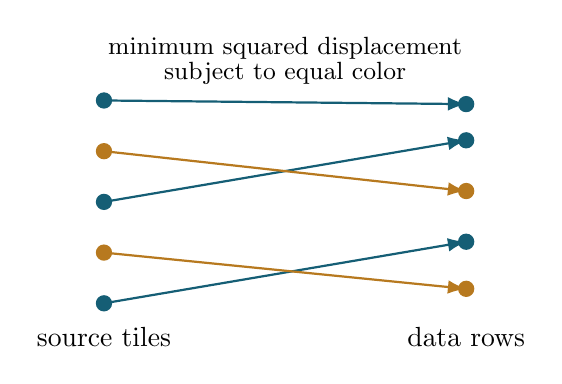
\begin{tikzpicture}[>=Latex,scale=0.92]
  \foreach \y/\col in {0/AimBlue,0.7/AimGold,1.4/AimBlue,2.1/AimGold,2.8/AimBlue}
    \fill[\col] (0,\y) circle (3.2pt);
  \foreach \x/\y/\col in {5/0.2/AimGold,5/0.85/AimBlue,5/1.55/AimGold,5/2.25/AimBlue,5/2.75/AimBlue}
    \fill[\col] (\x,\y) circle (3.2pt);
  \draw[AimBlue,thick,->] (0,0) -- (5,0.85);
  \draw[AimGold,thick,->] (0,0.7) -- (5,0.2);
  \draw[AimBlue,thick,->] (0,1.4) -- (5,2.25);
  \draw[AimGold,thick,->] (0,2.1) -- (5,1.55);
  \draw[AimBlue,thick,->] (0,2.8) -- (5,2.75);
  \node[below] at (0,-0.2) {source tiles};
  \node[below] at (5,-0.2) {data rows};
  \node[align=center] at (2.5,3.35)
    {\small minimum squared displacement\\[-1mm]\small subject to equal color};
\end{tikzpicture}
\end{center}

\subsection{What kind of OT is this?}

For two equally weighted empirical point clouds, the assignment is the
discrete quadratic-cost Monge solution.  It shortens conditional displacement
paths and reduces the kinetic burden on the learned vector field.  It also
chooses a consistent correspondence for an otherwise permutation-ambiguous
set.

There is an important scope qualification.  The assignment couples
\emph{tiles inside each sampled shape}, not complete examples across a
minibatch.  It is therefore an empirical, per-example OT coupling of colored
point clouds, rather than a direct computation of the global
\(W_2\)-optimal coupling between the full source law and the full data law.

\section{Flow matching for \texorpdfstring{\((x,y,\theta)\)}{(x,y,theta)}}

\subsection{Conditional displacement path}

Throughout this note we use a \term{linear time schedule}: training samples
\(t\sim\mathcal U[0,1]\), and sampling advances on a uniform grid in the same
variable \(t\).  For each OT-coupled pair \((G^0,G^1)\), the conditional path is
\[
  G_t=(1-t)G^0+tG^1,
  \qquad
  \dot G_t=G^1-G^0=:V^\star.
\]
The network receives \(t\) and predicts velocity with respect to \(t\).
Uniform time sampling gives equal training mass to equal-length subintervals
of the source-to-data path.

For L2 flow matching, the population-optimal predictor is the conditional
mean
\[
 v^\star(g,b,c,t,\ell)
 =\E\!\left[G^1-G^0\given G_t=g,B_t=b,C=c,T=t,\ell\right].
\]
Sampling solves the learned probability-flow ODE
\[
  \frac{dG_t}{dt}=v_\theta(G_t,B_t,C,t,\ell),\qquad G_0\sim q_0^G.
\]
Sampling uses explicit Euler steps on \(t_k=k/K\):
\[
  G_{t_{k+1}}=G_{t_k}
  +(t_{k+1}-t_k)\,v_\theta(G_{t_k},B_{t_k},C,t_k,\ell).
\]

\subsection{The angular coordinate}

The third coordinate is the scaled, wrapped angle
\[
  a=\frac{\sqrt3}{\pi}\operatorname{wrap}_{[-\pi,\pi)}(\theta).
\]
OT cost and interpolation treat \(a\) as an ordinary Euclidean coordinate.
The generated value is converted back by
\(\theta=a\pi/\sqrt3\) and wrapped only when decoded.
Thus the current method is simple and variance-balanced, but it does not use
the geodesic distance on \(S^1\): angles just below \(-\pi\) and just below
\(+\pi\) are physically close yet far apart in the assignment cost.

\section{Inness as a continuous-time Markov reveal process}

\subsection{Markov processes and hazard functions}

A stochastic process \((X_t)_{0\le t\le1}\) is \term{Markov} when its current
state contains all the information from the past that is relevant to its
future.  Formally, for \(0\le s<t\), every measurable set \(D\), and the
history \(\mathcal F_s=\sigma(X_r:0\le r\le s)\),
\[
  \Pp(X_t\in D\mid\mathcal F_s)
  =\Pp(X_t\in D\mid X_s).
\]
PenroseAim's reveal process is time-inhomogeneous: the law of the next jump
depends on the present time \(t\), as well as on the present state.

Let \(T\) be the reveal time of one probe.  Its survival function is
\(S(t)=\Pp(T>t)\).  The \term{hazard function} is the instantaneous reveal rate
conditional on having survived unrevealed up to time \(t\):
\[
  \lambda(t)
  =\lim_{h\downarrow0}
    \frac{\Pp(t<T\le t+h\mid T>t)}{h}.
\]
To derive it from \(S\), observe that the probability mass lost from the
surviving population over \((t,t+h]\) is \(S(t)-S(t+h)\).  Conditioning on
survival to \(t\) therefore gives
\[
\begin{aligned}
  \lambda(t)
  &=\lim_{h\downarrow0}
    \frac{S(t)-S(t+h)}{h\,S(t)}\\
  &=-\frac{S'(t)}{S(t)}
   =-\frac{d}{dt}\log S(t).
\end{aligned}
\]
Equivalently, the differential relation \(S'(t)=-\lambda(t)S(t)\), together
with \(S(0)=1\), integrates to
\[
  S(t)=\exp\!\left(-\int_0^t\lambda(s)\,ds\right).
\]
Thus
\[
  \Pp(t<T\le t+h\mid T>t)=\lambda(t)h+o(h).
\]
Writing the cumulative hazard as
\(\Lambda(t)=\int_0^t\lambda(s)\,ds\), the reveal probability is
\[
  \Pp(T\le t)=1-e^{-\Lambda(t)}.
\]
This language separates two aspects of a jump: the hazard determines
\emph{when} it occurs, while a mark distribution determines \emph{which value}
is written when it occurs.

\subsection{A uniform one-reveal clock for each probe}

Fix source bits \(B^0=(B^0_{ij})\) and clean endpoint bits
\(B^1=(B^1_{ij})\), where \(i\in\{1,\ldots,N\}\) indexes tiles and
\(j\in\{1,\ldots,m\}\) indexes the center/vertex probes of a tile.  Draw
independent reveal times
\[
  U_{ij}\sim\mathcal U[0,1],
\]
and introduce the reveal flag and current probe value
\[
  R_{ij}(t)=\1\{U_{ij}\le t\},\qquad
  B_{ij}(t)=
  \begin{cases}
    B_{ij}^0,&R_{ij}(t)=0,\\
    B_{ij}^1,&R_{ij}(t)=1.
  \end{cases}
\]
Every identified probe remains binary, has at most one reveal event, and is
frozen after that event.  A reveal need not produce a visible bit flip:
if \(B^0_{ij}=B^1_{ij}\), the flag changes while the displayed value does not.

For a uniform reveal time,
\[
  S(t)=\Pp(U_{ij}>t)=1-t,\qquad
  \Lambda(t)=-\log(1-t),\qquad
  \boxed{\lambda(t)=\frac{1}{1-t}}.
\]
The hazard increases because a probe still unrevealed late in the trajectory
must be forced to reveal before \(t=1\).  Although \(\lambda(t)\) diverges at
the endpoint, its construction is benign: \(U_{ij}<1\) almost surely, so every
probe is revealed by \(t=1\).

More generally, if a probe is still unrevealed at \(s<t\), then
\[
  \Pp(R_{ij}(t)=0\mid R_{ij}(s)=0)=\frac{1-t}{1-s},
  \qquad
  \Pp(R_{ij}(t)=1\mid R_{ij}(s)=0)=\frac{t-s}{1-s}.
\]
At training time, when only one randomly chosen \(t\) is needed, drawing
\(R_{ij}(t)\sim\Ber(t)\) directly has exactly the same one-time marginal as
drawing and retaining the full clock \(U_{ij}\).

\subsection{Why the reveal flag belongs to the Markov state}

The bit array \(B_t\) by itself does not record whether an unchanged bit has
already been revealed.  For example, observing \(B_{ij}(t)=1\) does not say
whether the probe is an unrevealed source \(1\), or a probe already revealed
to a clean endpoint \(1\).  Those cases have different futures: the former
can still undergo a reveal event, while the latter is frozen.

The correct state is therefore the augmented pair
\[
  X_t=(B_t,R_t)\in
  \{0,1\}^{N\times m}\times\{0,1\}^{N\times m}.
\]
Conditional on the clean endpoint \(B^1\), this augmented process is Markov.
The sampler implements precisely this augmentation by storing a Boolean
\code{revealed} tensor in addition to the current probe values.  The
Transformer does not receive \(R_t\), but the sampling process uses it to
prevent a second reveal.

\subsection{Infinitesimal generator of the endpoint bridge}

For an array \(b\), let \(b^{(i,j)\leftarrow q}\) mean ``replace entry
\((i,j)\) by \(q\) and leave every other entry unchanged''; define the same
operation for \(r\).  Conditional on \(B^1\), the generator of the reveal
bridge is
\[
\begin{aligned}
(\mathcal L_t^{B^1}f)(b,r)
&=
\sum_{i=1}^{N}\sum_{j=1}^{m}
\frac{\1\{r_{ij}=0\}}{1-t}\\
&\quad\times
\left[
 f\!\left(
 b^{(i,j)\leftarrow B^1_{ij}},
 r^{(i,j)\leftarrow1}
 \right)-f(b,r)
\right].
\end{aligned}
\]
This formula says that, over a short interval \([t,t+h]\), every unrevealed
pair \((i,j)\) reveals independently with probability
\(h/(1-t)+o(h)\); the probability of two specified probes revealing in that
same infinitesimal interval is \(o(h)\).  The destination is deterministic
when \(B^1\) is fixed.

\subsection{How tile-level inness evolves}

The generated inness of tile \(i\) is the probe average
\[
  \iota_i(t)=\frac1m\sum_{j=1}^m B_{ij}(t).
\]
It is a pure-jump process with increments in
\(\{-1/m,0,+1/m\}\).  Conditional on both endpoints,
\[
  \E[\iota_i(t)\mid B_i^0,B_i^1]
  =(1-t)\iota_i^0+t\iota_i^1.
\]
Thus its sample paths are step functions, while its conditional mean follows
the same linear interpolation as the geometry path.  Because the clocks are
independent,
\[
  \operatorname{Var}[\iota_i(t)\mid B_i^0,B_i^1]
  =\frac{t(1-t)}{m^2}
   \sum_{j=1}^m(B^1_{ij}-B^0_{ij})^2.
\]
Only probes whose endpoint differs from their source contribute visible
uncertainty; it is largest at \(t=1/2\) and vanishes at both endpoints.

There are \(m(1-t)\) unrevealed probes per tile in expectation.  Multiplying
by the per-probe hazard gives an expected total reveal intensity
\(m(1-t)/(1-t)=m\): under linear time, reveals are spread uniformly across
the trajectory in expectation.

This gives a precise meaning to ``diffusing inness.''  The soft scalar
training weight \(\omega_i\) is not itself diffused.  Rather, binary local
occupancy facts are progressively disclosed, and their average supplies the
generated tile opacity.

\begin{center}
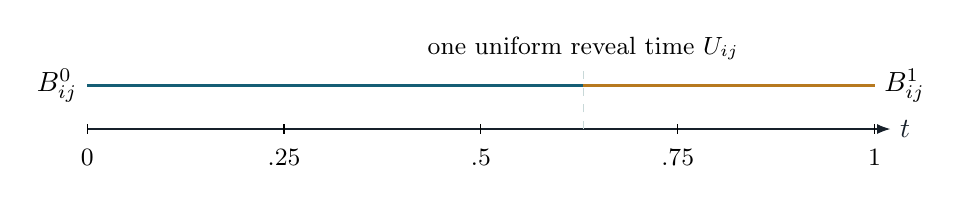
\begin{tikzpicture}[>=Latex,x=10cm,y=1cm]
  \draw[->,AimInk] (0,0) -- (1.02,0) node[right] {\(t\)};
  \foreach \x/\lab in {0/0,.25/{.25},.5/{.5},.75/{.75},1/1}
    \draw (\x,0.06)--(\x,-0.06) node[below=2pt] {\small\(\lab\)};
  \draw[very thick,AimBlue] (0,0.55)--(.63,0.55);
  \draw[very thick,AimGold] (.63,0.55)--(1,0.55);
  \draw[dashed,AimRule] (.63,0)--(.63,0.75);
  \node[left] at (0,0.55) {\(B^0_{ij}\)};
  \node[right] at (1,0.55) {\(B^1_{ij}\)};
  \node[above] at (.63,0.75) {\small one uniform reveal time \(U_{ij}\)};
\end{tikzpicture}
\end{center}

\subsection{Learned generative jump law}

During generation, thresholds \(U_{ij}\) and flags \(R_{ij}\) are sampled
once.  When probe \((i,j)\) becomes newly revealed, the sampler draws
\[
  B_{ij}\sim
  \Ber\!\left(\sigmoid\eta_{\theta,ij}
  (G_t,B_t,C,t,\ell)\right)
\]
and never changes that coordinate again.  In an ideal infinitesimal
description, write
\[
 q_{\theta,ij}(q\mid g,b,C,t,\ell)
 =\Pp_\theta(B_{ij}=q\mid g,b,C,t,\ell),
 \qquad q\in\{0,1\}.
\]
The learned marked-jump generator is then
\[
\begin{aligned}
(\mathcal L_t^\theta f)(g,b,r)
&=\sum_{i=1}^{N}\sum_{j=1}^{m}
\frac{\1\{r_{ij}=0\}}{1-t}
\sum_{q\in\{0,1\}}q_{\theta,ij}(q\mid g,b,C,t,\ell)\\
&\quad\times
\left[
f\!\left(g,b^{(i,j)\leftarrow q},r^{(i,j)\leftarrow1}\right)
-f(g,b,r)
\right].
\end{aligned}
\]
Together with the continuous geometry flow, the full generator is
\[
  (\mathcal A_t^\theta f)(g,b,r)
  =\left\langle\nabla_g f,\,
    v_\theta(g,b,C,t,\ell)\right\rangle
   +(\mathcal L_t^\theta f)(g,b,r).
\]
This equation is the most compact mathematical description of PenroseAim:
a deterministic drift coupled bidirectionally through the Transformer to
discrete, time-inhomogeneous jumps.

\section{Training objective}

Let \(\ell_p(r)=|r|\) for the configured L1 option and
\(\ell_p(r)=r^2\) for the default L2 option.  The geometry term is weighted by
the target soft inness:
\[
\mathcal L_{\mathrm{geom}}(\theta)
=
\E\!\left[
\frac{
\sum_{i=1}^N\omega_i
\sum_{d=1}^3
\ell_p\!\left(v_{\theta,id}-V^\star_{id}\right)}
{3\sum_{i=1}^N\omega_i}
\right].
\]
Interior tiles therefore influence geometry more strongly, while the
normalization keeps the scale stable as total inness varies.

The probe head predicts the clean endpoint at every sampled time:
\[
\mathcal L_{\mathrm{probe}}(\theta)
=
\E\!\left[
-\frac1{Nm}\sum_{i,j}
\left\{
b^1_{ij}\log\sigma(\eta_{\theta,ij})
+(1-b^1_{ij})\log[1-\sigma(\eta_{\theta,ij})]
\right\}
\right].
\]
The total objective is
\[
  \boxed{\quad
  \mathcal L(\theta)=
  \mathcal L_{\mathrm{geom}}(\theta)
  +\lambda_{\mathrm{in}}\mathcal L_{\mathrm{probe}}(\theta),
  \qquad \lambda_{\mathrm{in}}=0.25\ \text{by default}.
  \quad}
\]

This is \emph{clean-endpoint denoising classification}, not explicit
likelihood training of transition intensities.  The reveal hazard is fixed
analytically; only the Bernoulli mark distribution is learned.

\section{One training draw and one generated trajectory}

\subsection{Training}
\begin{enumerate}
  \item Sample a shape mask, construct its transformed tiling, and retain the
        top \(N\) tiles by soft inness.
  \item Sample independent geometry and probe nulls.
  \item Solve color-constrained LSA in \((x,y,a)\), then permute both null
        geometry and null probes.
  \item Draw \(t\sim\mathcal U[0,1]\), linearly interpolate geometry, and
        independently reveal each target probe with probability \(t\).
  \item Predict \(V^\star=G^1-G^0\) and clean \(B^1\); optimize weighted
        geometry error plus binary cross-entropy.
\end{enumerate}

\subsection{Generation}
\begin{enumerate}
  \item Draw \(G_0\) from the geometry null, \(B_0\) from the fitted
        one-inflated null, and independent probe reveal thresholds.
  \item March over the linear grid \(t_k=k/K\).
  \item At each step, Euler-update geometry and sample every newly revealed
        probe once from the model's current clean logits.
  \item Decode \(a\) to wrapped \(\theta\); render opacity from the mean of
        generated probe bits.
\end{enumerate}

\begin{figure}[ht]
\centering
\begin{minipage}[t]{0.46\linewidth}
\centering
\includegraphics[height=5.0cm]{assets/bat_flow_start.pdf}\\[-1mm]
\small Early trajectory state
\end{minipage}\hfill
\begin{minipage}[t]{0.46\linewidth}
\centering
\includegraphics[height=5.0cm]{assets/bat_flow_end.pdf}\\[-1mm]
\small Final trajectory state
\end{minipage}
\caption{A stored 200-step hexagonal ``bat'' trajectory from the
\code{aim\_0815\_0611\_128x8\_t120\_l2} checkpoint.  Position and orientation
move continuously; opacity is quantized in units of \(1/7\) because a hexagon
has seven identified probes.}
\end{figure}

\section{Interpretive cautions}

\begin{enumerate}
  \item \textbf{``Reverse sampling'' runs source to data.}
        The function name follows diffusion convention, but its integration
        direction is \(t:0\to1\), from null to shaped tiling.

  \item \textbf{The Markov state includes reveal flags.}
        Generation tracks these flags internally, but the Transformer is given
        only the current bits, not the flags.  A bit that was revealed to the
        same value is observationally indistinguishable from an unrevealed bit.

  \item \textbf{Finite steps batch jumps.}
        In continuous time, simultaneous thresholds have probability zero.
        In one Euler interval, several probes can be sampled independently
        from logits produced by a single network evaluation.  This approaches
        the sequential marked-jump picture as the step size decreases.

  \item \textbf{OT ignores inness in its cost.}
        Matching uses only \((x,y,a)\) and color.  Probe nulls follow the
        geometry permutation, but neither target soft inness nor target probe
        patterns influence the assignment.

  \item \textbf{Angle is Euclidean during training.}
        The representation has the correct uniform variance but not the
        circular geodesic near the wrap boundary.

  \item \textbf{The joint process is coupled by the network.}
        Although the prescribed reveal clocks are independent, predicted probe
        probabilities depend on all tiles and on the evolving geometry;
        geometry velocity simultaneously depends on current probe bits.
\end{enumerate}

\section{Implementation correspondence}

\begin{tabularx}{\linewidth}{@{}>{\ttfamily}p{0.31\linewidth}X@{}}
\toprule
\normalfont\textbf{Location} & \textbf{Mathematical role}\\
\midrule
PenroseSpur/sampler.py &
Data construction, \(a=(\sqrt3/\pi)\theta\), probe evaluation, top-\(N\)
selection, and source geometry law.\\
PenroseSpur/match.py &
Quadratic cost, color-restricted exact LSA, and source permutation.\\
PenroseAim/null\_inness.py &
One-inflated binomial fit, cache, and probe-null sampler.\\
PenroseAim/sampler.py &
OT-coupled path construction, Bernoulli reveals, Euler flow, and trajectory
decoding; this note adopts a linear time schedule.\\
PenroseAim/losses.py &
Target-inness-weighted velocity loss and clean-probe BCE.\\
PenroseAim/model.py &
Permutation-compatible Direct Transformer producing velocity and logits.\\
\bottomrule
\end{tabularx}

\section{Summary}

PenroseAim places two generative mechanisms on a shared tile-token state:
\[
\boxed{
\begin{aligned}
  dG_t &= v_\theta(G_t,B_t,C,t,\ell)\,dt,\\
  (B_t,A_t) &\text{ follows marked jumps at rate }(1-t)^{-1}.
\end{aligned}}
\]
The geometry endpoints are coupled by exact color-constrained empirical OT,
then connected by straight displacement paths for conditional flow matching.
The inness endpoint is represented by local binary occupancy probes and
reached through randomized progressive revelation.  A single Transformer
couples the two: current occupancy informs geometric motion, and current
geometry informs the clean-probe posterior.

The result is neither a conventional stochastic diffusion nor merely a
deterministic flow.  It is a compact hybrid PDMP whose continuous and discrete
parts share an OT-aligned tokenization and a common path-time clock.

\begin{thebibliography}{9}
\small
\bibitem{lipman2023}
Y.~Lipman, R.~T.~Q. Chen, H.~Ben-Hamu, M.~Nickel, and M.~Le.
\newblock Flow Matching for Generative Modeling.
\newblock \emph{International Conference on Learning Representations}, 2023.

\bibitem{tong2024}
A.~Tong, K.~Fatras, N.~Malkin, G.~Huguet, Y.~Zhang, J.~Rector-Brooks,
G.~Wolf, and Y.~Bengio.
\newblock Improving and Generalizing Flow-Based Generative Models with
Minibatch Optimal Transport.
\newblock \emph{Transactions on Machine Learning Research}, 2024.

\bibitem{villani2009}
C.~Villani.
\newblock \emph{Optimal Transport: Old and New}.
\newblock Springer, 2009.

\bibitem{davis1993}
M.~H.~A. Davis.
\newblock \emph{Markov Models and Optimization}.
\newblock Chapman \& Hall, 1993.
\end{thebibliography}

\end{document}
